\chapter{Revolution, the Korean War and a Divided Region}

\section{1945: the postwar settlement}

Japan's defeat left a vacuum. Within five years East Asia was divided along Cold War
lines that still exist: two Chinas, two Koreas, and a Japan aligned with the United States.

\begin{center}
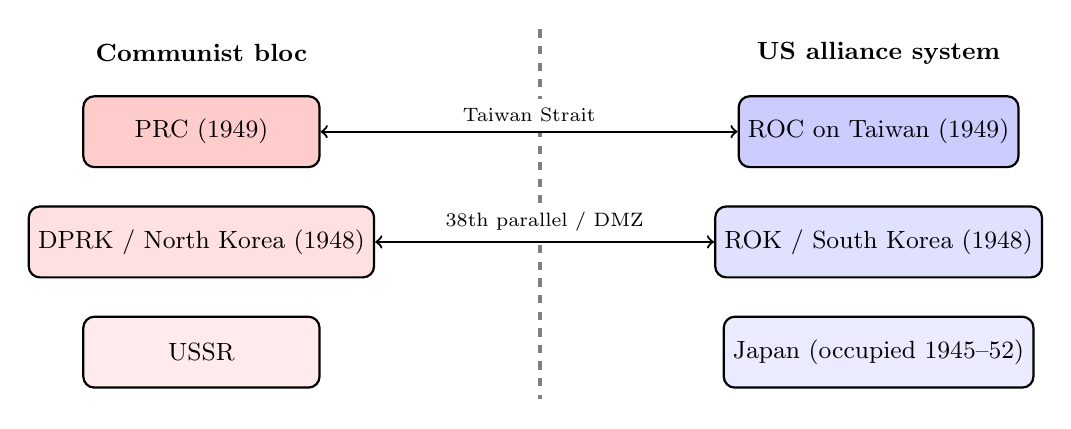
\begin{tikzpicture}[b/.style={draw, thick, rounded corners, align=center, font=\small, minimum width=3cm, minimum height=0.9cm}]
  \node[font=\small\bfseries] at (-4.3,3.2) {Communist bloc};
  \node[font=\small\bfseries] at (4.3,3.2) {US alliance system};
  \node[b, fill=red!20] (prc) at (-4.3,2.2) {PRC (1949)};
  \node[b, fill=red!12] (dprk) at (-4.3,0.8) {DPRK / North Korea (1948)};
  \node[b, fill=red!8] (ussr) at (-4.3,-0.6) {USSR};
  \node[b, fill=blue!20] (roc) at (4.3,2.2) {ROC on Taiwan (1949)};
  \node[b, fill=blue!12] (rok) at (4.3,0.8) {ROK / South Korea (1948)};
  \node[b, fill=blue!8] (jp) at (4.3,-0.6) {Japan (occupied 1945--52)};
  \draw[very thick, dashed, gray] (0,3.5) -- (0,-1.2);
  \draw[<->, thick] (prc) -- node[above, font=\scriptsize, fill=white] {Taiwan Strait} (roc);
  \draw[<->, thick] (dprk) -- node[above, font=\scriptsize, fill=white] {38th parallel / DMZ} (rok);
\end{tikzpicture}
\end{center}

\section{China: civil war and the People's Republic}

\subsection{Why did the Communists win?}

The KMT--CCP civil war resumed in 1946. Despite US aid to the Nationalists, the CCP won by
1949. Standard explanations (know at least three):

\begin{enumerate}
  \item The war with Japan had exhausted and discredited the KMT (corruption,
        hyperinflation, heavy conscription), while the CCP built rural bases and gained
        prestige as patriotic resisters.
  \item \textbf{Land reform}: the CCP redistributed land from landlords to peasants in
        areas it controlled, gaining support and recruits.
  \item \textbf{Mao's strategy}: peasant-based revolution and guerrilla warfare
        (``the countryside surrounds the cities''), rather than the Soviet model of an
        urban workers' uprising.
  \item Military decisions: KMT armies overextended into Manchuria and collapsed in the
        Huaihai campaign (1948--49).
\end{enumerate}

On 1 October 1949 Mao Zedong proclaimed the People's Republic of China (\zh{中华人民共和国})
from Tiananmen. Chiang Kai-shek and about two million followers retreated to Taiwan, where
the Republic of China continued under martial law until 1987.

\subsection{The Mao era (1949--1976)}

\begin{center}
\begin{tabular}{lp{10.5cm}}
\toprule
Years & Campaign and effects \\
\midrule
1950--53 & land reform (violent; perhaps 1--2 million landlords killed); Korean War;
marriage law (1950) banning arranged marriage and concubinage \\
1953--57 & first Five-Year Plan (Soviet model, heavy industry); collectivization \\
1956--57 & Hundred Flowers campaign invites criticism; Anti-Rightist campaign punishes
critics \\
1958--62 & \textbf{Great Leap Forward}: people's communes, backyard furnaces, inflated
grain reports; resulting famine killed an estimated 30 million or more \\
1966--76 & \textbf{Cultural Revolution}: Mao mobilizes Red Guards against ``capitalist
roaders'' and the ``four olds'' (old customs, culture, habits, ideas); temples, books and
the Confucius family cemetery attacked; schools closed; millions persecuted; youths ``sent
down'' to the countryside \\
1972 & Nixon visits China; US--China rapprochement \\
1976 & Mao dies; the ``Gang of Four'' arrested \\
\bottomrule
\end{tabular}
\end{center}

\begin{aside}
The Cultural Revolution's attack on Confucius (the 1973--74 ``Criticize Lin Biao,
Criticize Confucius'' campaign) is a striking contrast with today's PRC, which funds
Confucius Institutes abroad and celebrates traditional culture. The professor used this as
an example of how ``tradition'' is constantly re-evaluated for present political purposes.
\end{aside}

\section{Korea: liberation and division}

\subsection{Division at the 38th parallel}

In August 1945 two US officers, working late at night with a National Geographic map,
proposed the 38th parallel as a line dividing Soviet and American zones of occupation in
Korea. It was meant to be temporary. Plans for a trusteeship and joint elections failed.

\begin{itemize}
  \item South: the \textbf{Republic of Korea} (\ko{대한민국}, Daehan Minguk), August 1948,
        under \textbf{Syngman Rhee}, a long-time exile in the US. The US military government
        had retained many colonial-era officials and police.
  \item North: the \textbf{Democratic People's Republic of Korea} (\ko{조선민주주의인민공화국}),
        September 1948, under \textbf{Kim Il-sung}, a former anti-Japanese guerrilla
        backed by the Soviets.
\end{itemize}

\begin{remark}
Note the names: the South uses \emph{Han} (\ko{한국}), the North uses \emph{Joseon}
(\ko{조선}). Even the word for ``Korea'' depends on which side you are on.
\end{remark}

\subsection{The Korean War (1950--1953)}

\begin{center}
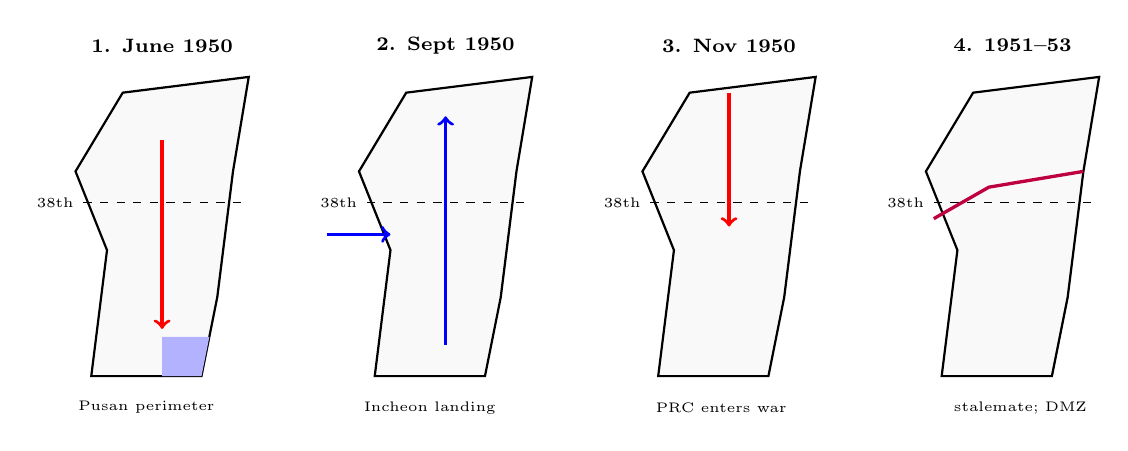
\begin{tikzpicture}[x=1cm, y=1cm]
  \foreach \i/\title in {0/{1. June 1950}, 1/{2. Sept 1950}, 2/{3. Nov 1950}, 3/{4. 1951--53}} {
    \begin{scope}[xshift=\i*3.6cm]
      \draw[thick, fill=gray!5] (0,0) -- (0.2,1.6) -- (-0.2,2.6) -- (0.4,3.6) -- (2.0,3.8)
          -- (1.8,2.6) -- (1.6,1.0) -- (1.4,0) -- cycle;
      \node[font=\scriptsize\bfseries] at (0.9,4.2) {\title};
      \draw[dashed] (-0.1,2.2) -- (1.9,2.2);
      \node[font=\tiny, anchor=east] at (-0.1,2.2) {38th};
    \end{scope}
  }
  % 1: invasion
  \draw[->, very thick, red] (0.9,3.0) -- (0.9,0.6);
  \fill[blue!30] (0.9,0.0) -- (1.4,0) -- (1.5,0.5) -- (0.9,0.5) -- cycle;
  \node[font=\tiny, align=center] at (0.7,-0.4) {Pusan perimeter};
  % 2: Inchon landing
  \draw[->, very thick, blue] (3.0,1.8) -- (3.8,1.8);
  \draw[->, very thick, blue] (4.5,0.4) -- (4.5,3.3);
  \node[font=\tiny] at (4.3,-0.4) {Incheon landing};
  % 3: Chinese intervention
  \draw[->, very thick, red] (8.1,3.6) -- (8.1,1.9);
  \node[font=\tiny, align=center] at (8.0,-0.4) {PRC enters war};
  % 4: stalemate
  \draw[very thick, purple] (10.7,2.0) -- (11.4,2.4) -- (12.6,2.6);
  \node[font=\tiny, align=center] at (11.8,-0.4) {stalemate; DMZ};
\end{tikzpicture}
\end{center}

\begin{enumerate}
  \item \textbf{25 June 1950}: North Korean forces, with Stalin's approval, invaded the
        South and nearly overran it; UN forces held only the Pusan (Busan) perimeter.
  \item \textbf{September 1950}: General MacArthur's amphibious landing at Incheon cut North
        Korean lines; UN forces crossed the 38th parallel and advanced toward the Yalu
        river.
  \item \textbf{October--November 1950}: China entered the war with hundreds of thousands
        of ``People's Volunteers'', pushing UN forces back south of Seoul.
  \item \textbf{1951--1953}: stalemate near the 38th parallel while armistice talks
        dragged on (the main issue was repatriation of prisoners). Armistice signed
        \textbf{27 July 1953}; no peace treaty has ever been signed.
\end{enumerate}

\begin{important}[Consequences]
\begin{itemize}
  \item About 3 million dead, mostly Korean civilians; nearly every city levelled; millions
        of separated families.
  \item The division hardened: the Demilitarized Zone (DMZ) remains one of the most
        militarized borders on earth.
  \item The US committed to defending Taiwan and stationed troops in South Korea and Japan.
  \item Japan's economy boomed from US procurement orders (``a gift from the gods'',
        said PM Yoshida).
  \item Canada sent over 26\,000 troops; 516 Canadians died. (Our professor pointed out the
        Korean War memorials in Ottawa and Brampton.)
\end{itemize}
\end{important}

\section{Japan: occupation and the ``reverse course''}

The US-led occupation under General Douglas MacArthur (SCAP) lasted from 1945 to 1952.

\begin{itemize}
  \item \textbf{Demilitarization and democratization}: the army and navy dissolved; war
        crimes trials (Tokyo Tribunal); purge of militarists; land reform; breakup of the
        \emph{zaibatsu} conglomerates; women's suffrage (1946); labour unions legalized.
  \item \textbf{The 1947 Constitution}: drafted largely by SCAP staff. The emperor became
        ``the symbol of the State and of the unity of the people''; sovereignty rests with
        the people. \textbf{Article 9} renounces war and the maintenance of armed forces.
  \item Emperor Hirohito was not tried; he renounced his divinity (January 1946) and
        toured the country as a ``human emperor''.
  \item \textbf{Reverse course} (from 1947--48): with the Cold War, the US prioritized
        Japan's economic recovery and anti-communism; purged conservatives returned; the
        Self-Defense Forces were created (1954) despite Article 9.
  \item San Francisco Peace Treaty and US--Japan Security Treaty (1951, effective 1952).
        Okinawa remained under US control until 1972.
\end{itemize}

\section{Divided nations compared}

\begin{center}
\begin{tabular}{lp{5.5cm}p{5.5cm}}
\toprule
 & China / Taiwan & North / South Korea \\
\midrule
Origin of division & civil war (1946--49) & Soviet--US occupation zones (1945), war 1950--53 \\
Political systems & one-party PRC; Taiwan democratized from 1987 & DPRK dynastic one-party state; ROK democratized from 1987 \\
Recognition & most states recognize PRC (Canada in 1970) & both UN members since 1991 \\
Contact today & heavy trade and travel & almost none; occasional summits \\
\bottomrule
\end{tabular}
\end{center}

\section*{Summary}
\begin{itemize}
  \item The CCP won the civil war (land reform, peasant mobilization, KMT failures); the PRC
        was founded on 1 October 1949; the ROC retreated to Taiwan.
  \item The Mao era: land reform, Great Leap Forward famine, Cultural Revolution.
  \item Korea was divided at the 38th parallel in 1945; the Korean War (1950--53) ended in
        an armistice, not peace.
  \item The US occupation remade Japan (1947 Constitution, Article 9), then reversed course
        to build an anti-communist ally.
\end{itemize}
